\documentclass{beamer}
\usepackage[utf8]{inputenc}
\usepackage[authoryear]{natbib}
\usepackage{subfigure}
\usepackage[noend]{algpseudocode}
\usepackage{color}
\usepackage{alltt}
\usepackage{tabularx}
\usepackage{amsmath,amssymb}
\usepackage{microtype}
\usepackage{tikz}
\usetikzlibrary{fit,positioning}

\setbeamertemplate{navigation symbols}{} 

\usepackage{multimedia}

%\usetheme{none}
%\usecolortheme{albatross}

\newenvironment{centercolumns}{\begin{columns}[c]}{\end{columns}}
%\newcommand{\newblock}{}


\newcommand{\dataset}{\mathcal{D}}
\newcommand{\model}{\mathcal{M}}
\newcommand{\parameters}{\theta}
\newcommand{\vparameters}{\phi}
\newcommand{\vy}{\mathbf{y}}
\newcommand{\vx}{\mathbf{x}}
\newcommand{\diff}{\mathrm{d}}

\title{Probabilistic models for big data}
\author{Antti Honkela and Arto Klami}
\date{24 October 2014}



\begin{document}

\frame{\titlepage}

%\frame{\frametitle{Outline} \tableofcontents}

\section{Introduction}

\begin{frame}
  \frametitle{Probabilistic modelling and big data}

  \begin{itemize}
  \item New kind of thinking: data as a resource, we do not need to
    use it all if less is enough to solve the problem
  \item Aim: getting below $\mathcal{O}(n)$ complexity for $n$ samples
  \item The results are by definition approximations
  \item Increasing bias to decrease variance over finite time
  \end{itemize}
\end{frame}

\begin{frame}
  \frametitle{Disclaimer}

  \begin{itemize}
  \item This presentation is based on our cursory reading of papers we
    selected in the summer for our ``Seminar in Probabilistic Models
    for Big Data''
  \item It is probable there are errors in our interpretations
    \begin{itemize}
    \item \textbf{If you are interested in the topic, please read the
      papers yourself before drawing strong conclusions!}
    \end{itemize}
  \end{itemize}
\end{frame}

\begin{frame}
  \frametitle{For which models are the methods applicable?}
\end{frame}

\section{VB}

\begin{frame}
  \frametitle{Variational inference basics}

  \begin{itemize}
  \item Idea: approximate the posterior distribution $p(\parameters | \dataset)$
    with another distribution $q(\parameters)$ that is analytically tractable
  \item Learn the approximation by minimizing the distance between $q(\parameters)$ and $p(\parameters | \dataset)$
  \item The distance is measured by the Kullback-Leibler divergence
    $D(q||p) = \int q(\parameters) \log \frac{q(\parameters)}{p(\parameters| \dataset)}\diff \parameters$
  \item ...and the minimization is often converted into maximizing a lower bound on the marginal
    likelihood (ELBO):
    $L = \int q(\parameters) \log \frac{p(\dataset,\parameters)}{q(\parameters)} \diff \parameters= p(\dataset) - D(q||p)$
  \item Predictions then made by replacing $\int p(\vx|\parameters) p(\parameters | \dataset) \diff \parameters$ by
    $\int p(\vx|\parameters) q(\parameters) \diff \parameters$
  \end{itemize}
\end{frame}

\begin{frame}
  \frametitle{Mean-field variational inference}

  \begin{itemize}
    \item Often $q(\parameters)$ is factorized as $\prod_i q(\parameters_i)$, so that
      we can optimize one factor at a time
    \item Differentiating wrt to $q(\parameters_i)$ and setting the derivative to zero provides a closed-form
      update $\log q(\parameters_i) = \int q(\parameters_{-i}) \log p(\dataset, \parameters) \diff \parameters_{-i} + C$
    \item The expectation over all other factors is typically easy to compute for exponential
      family distributions with conjugate priors (and much harder for everything else)
    \item Leads to an algorithm closely resembling expectation maximization
  \end{itemize}
\end{frame}

\begin{frame}
  \frametitle{Towards more scalable variational inference}

  \begin{itemize}
  \item Given a parametric form $q(\parameters|\vparameters)$ VB is an optimization problem:
  $L(\vparameters) = \int q(\parameters|\vparameters) \log \frac{p(\dataset,\parameters)}{q(\parameters|\vparameters)} \diff \parameters$
  \item Gradient-based optimization generally applicable: $\vparameters \leftarrow \vparameters + \delta
    \nabla L(\vparameters)$
  \item Natural gradient speeds up convergence: Replace $\nabla L(\vparameters)$ with $F^{-1}(\vparameters)
\nabla L(\vparameters)$, where $F(\vparameters)$ is the Fisher information matrix
  consisting of expectations of second derivatives of $\log q(\parameters | \vparameters)$
 (Honkela et al., JMLR 2010)
  \item Stochastic gradients applicable (Hoffman et al., JMLR 2013); more about this during the seminar
  \end{itemize}
\end{frame}

\begin{frame}
  \frametitle{Variational inference example}

  \begin{figure}
  \begin{center}
  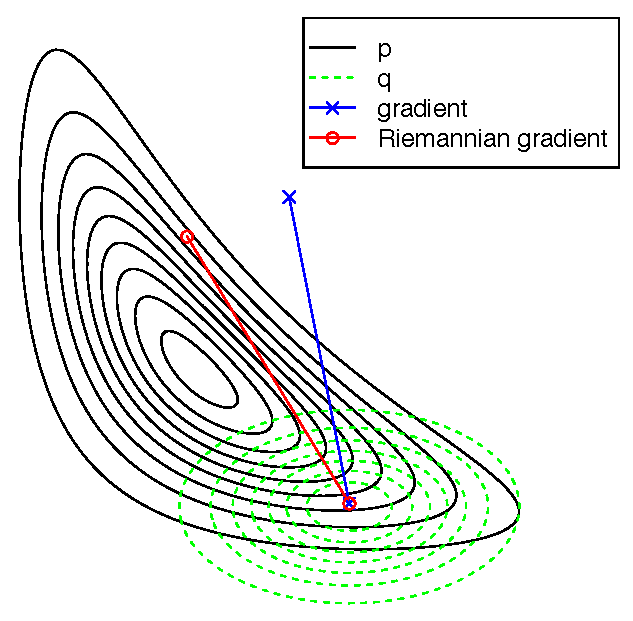
\includegraphics[width=0.7\textwidth]{VBnatgrad.pdf}
  \end{center}
  \end{figure}
  \vfill \hfill {\tiny Figure from Honkela et al. (JMLR 2010)}
\end{frame}

\begin{frame}
  \frametitle{Stochastic variational inference}

  \begin{enumerate}
  \item M.D. Hoffman, D.M. Blei, C. Wang, J. Paisley. \textbf{Stochastic Variational Inference}, JMLR 2013
  \item R. Ranganath, C. Wang, D.M. Blei, E. Xing, \textbf{An Adaptive Learning Rate for Stochastic Variational Inference}, ICML 2013.
  \end{enumerate}
\end{frame}

\begin{frame}
  \frametitle{Doubly stochastic VB}

  \begin{enumerate}
  \item M. Titsias, M. Lazaro-Gredilla, \textbf{Doubly Stochastic Variational Bayes for non-Conjugate Inference}, ICML 2014.
  \end{enumerate}

  \begin{itemize}
  \item Stochastic gradient by sampling from the posterior
    approximation $q(\parameters)$ allows avoiding evaluating difficult
    integrals
  \item Posterior approximation as affine transformation of a standard
    distribution
  \item Can be combined with subsampling data for SVI
  \end{itemize}
\end{frame}

\begin{frame}
  \frametitle{Stochastic VB for deep learning}

  \begin{enumerate}
  \item D.J. Rezende, S. Mohamed, D. Wierstra, \textbf{Stochastic Backpropagation and Approximate Inference in Deep Generative Models}, ICML 2014.
  \end{enumerate}

  \begin{itemize}
  \item Algorithmic similarities with Titsias \& Lazaro-Gredilla
  \item Layered deep neural network model
    \begin{itemize}
    \item Latent variables at every layer
    \item Point estimates for network weights
    \end{itemize}
  \item Use another deep neural network model to parametrise
    the posterior approximation for latent variables
  \end{itemize}
\end{frame}

\begin{frame}
  \frametitle{Big data GPs}

  \begin{enumerate}
  \item J. Hensman, N. Fusi, N.D. Lawrence, \textbf{Gaussian Processes for Big Data}, UAI 2013.
  \end{enumerate}

  \begin{itemize}
  \item GP inference
    $$ y_i = f(\vx_i) + \epsilon $$
  \item Variational sparse GPs: introduce \emph{inducing variables}
    $$ \mathbf{u} = [f(\mathbf{z}_i)]_{i=1}^m $$
  \item Standard variational GPs collapse $\mathbf{u}$, but that
    cannot be done with SVI
  \end{itemize}
\end{frame}

\begin{frame}
  \frametitle{SVI for binary matrix factorisation}

  \begin{enumerate}
  \item J. M. Hernandez-Lobato, N. Houlsby, Z. Ghahramani, \textbf{Stochastic Inference for Scalable Probabilistic Modeling of Binary Matrices}, ICML 2014.
  \end{enumerate}

  \begin{itemize}
  \item Subsample both data points and ``global variables''
  \item Nice method for deciding mini-batch size
  \end{itemize}
\end{frame}

\section{Other}

\begin{frame}
  % Arto + Antti
  \frametitle{Stochastic gradients in general}

  \begin{enumerate}
  \item M. Schmidt, N. Le Roux, F. Bach, \textbf{Minimizing Finite Sums with the Stochastic Average Gradient}, arXiv 2013.
  \end{enumerate}
  \begin{itemize}
  \item Basic idea: introduce a memory of gradients and simply update the
    component from one data point or mini-batch at a time
  \item Improves the asymptotic convergence rate
  \end{itemize}

\end{frame}


\section{MCMC}

% Antti

\begin{frame}
  % Antti
  \frametitle{Approximate inference by sampling}

  \begin{itemize}
  \item A lot of Bayesian inference boils down to computing integrals
    $$ E[f(\parameters)] = \int_\parameters f(\parameters) p(\parameters | \dataset) \diff\parameters $$
    \begin{itemize}
    \item Model predictions, posterior statistics of parameters, \dots
    \end{itemize}
  \item $\parameters$ is often high-dimensional which makes these very difficult
  \item Stochastic approximation:
    $$ E[f(\parameters)] \approx \frac{1}{N} \sum_{i=1}^N f(\parameters_i), $$
    when $\parameters_i \sim p(\parameters | \dataset)$
  \item How to simulate samples following a given distribution?
  \end{itemize}
\end{frame}

\begin{frame}
  \frametitle{MCMC basics (Metropolis et al., 1953; Hastings, 1970)}

  \begin{itemize}
  \item Idea: construct a Markov chain, whose stationary distribution
    is the distribution of interest $p(\parameters | \dataset)$
  \item Requires an \emph{unnormalised} $p^*(\parameters | \dataset) \propto
    p(\parameters | \dataset)$
  \item In the Bayesian setting typically
    $$ p(\parameters | \dataset) = \frac{p(\dataset | \parameters) p(\parameters)}{p(\dataset)} $$
    which easily yields the unnormalised density
    $$ p^*(\parameters | \dataset) = p(\dataset | \parameters) p(\parameters) $$
  \item To define the Markov chain, we need to specify a transition
    distribution $q(\parameters' | \parameters)$
  \item The Markov chain is guaranteed to converge if it satisfies
    sufficient regularity conditions and the \emph{detailed balance}
    condition
    $$ q(\parameters' | \parameters) p(\parameters | \dataset) =
       q(\parameters | \parameters') p(\parameters' | \dataset) $$
  \end{itemize}
\end{frame}

\begin{frame}
  \frametitle{Metropolis--Hastings algorithm}

  \begin{itemize}
  \item The most widely used MCMC algorithm is the Metropolis--Hastings
    algorithm
  \item Accept--reject mechanism, proposals are accepted with probability
    $$ f(\parameters' | \parameters) = \min\left(1, \frac{\color{blue}q(\parameters | \parameters') p(\parameters' | \dataset)}
      {\color{red}q(\parameters' | \parameters) p(\parameters | \dataset)} \right) $$
  \item This satisfies the detailed balance because
    \begin{align*}
      {\color{red}f(\parameters' | \parameters)
      q(\parameters' | \parameters) p(\parameters | \dataset)}
      &= \min({\color{blue}q(\parameters' | \parameters) p(\parameters | \dataset)},
      {\color{red}q(\parameters | \parameters') p(\parameters' | \dataset)}) \\
      &= \min({\color{red}q(\parameters | \parameters') p(\parameters' | \dataset)},
      {\color{blue}q(\parameters' | \parameters) p(\parameters | \dataset)}) \\
      &= {\color{blue}f(\parameters | \parameters')
      q(\parameters | \parameters') p(\parameters' | \dataset)}
    \end{align*}
  \end{itemize}
\end{frame}

\begin{frame}
  % Antti
  \frametitle{Gradients in MCMC}
  % HMC etc

  \begin{itemize}
  \item Standard MCMC is based on proposal distributions whose shape is
    essentially \emph{independent of the target}
    \begin{itemize}
    \item E.g.~fixed multivariate Gaussian proposals
    \end{itemize}
  \item Target distribution gradients would allow utilising local shape
  \item Common algorithms:
    \begin{itemize}
    \item Langevin dynamics MCMC
    \item Hamiltonian Monte Carlo  (a.k.a. hybrid Monte Carlo)
    \end{itemize}
  \item Both based on constructing a suitable dynamical system and
    simulating it
  \end{itemize}
\end{frame}

\begin{frame}
  \frametitle{Langevin and Hamiltonian dynamics in MCMC}

  Langevin dynamics proposal:
  $$ \parameters^* = \parameters + \frac{\epsilon}{2} \nabla_\parameters p(\dataset, \parameters) + N(0, \epsilon I) $$
  \begin{itemize}
  \item Acceptance rate tends to one as $\epsilon \rightarrow 0$
  \end{itemize}
  \mbox{}\\
  Hamiltonian MCMC:
  \begin{itemize}
  \item Construct a Hamiltonian dynamical system with momentum
  \item Hamiltonian ($\approx$ ``energy'') is conserved in simulation
  \item Can take arbitrarily long steps, assuming the Hamiltonian
    system can be simulated accurately
    \begin{itemize}
    \item Symplectic geometry studies this problem
    \end{itemize}
  \end{itemize}
\end{frame}

\begin{frame}[allowframebreaks]
  % Arto + Antti
  \frametitle{MCMC: Stochastic gradients}

  \begin{enumerate}
  \item S. Ahn, A. Korattikara, M. Welling, \textbf{Bayesian posterior sampling via stochastic gradient Fisher scoring}, ICML 2012 and M. Welling, Y.W.Teh, \textbf{Bayesian Learning via Stochastic Gradient Langevin Dynamics}, ICML 2011.
  \item S. Patterson, Y. W. Teh, \textbf{Stochastic Gradient Riemannian Langevin Dynamics on the Probability Simplex}, NIPS 2013.
  \item S. Ahn, B. Shahbaba, M. Welling, \textbf{Distributed stochastic gradient MCMC}, ICML 2014.
  \end{enumerate}
\end{frame}


\begin{frame}
  \frametitle{MCMC: Stochastic gradients HMC}

  \begin{enumerate}
  \item T. Chen, E. Fox, C. Guestrin, \textbf{Stochastic Gradient Hamiltonian Monte Carlo}, ICML 2014.
  \end{enumerate}
  
  \begin{itemize}
  \item Naive introduction of stochastic gradients to HMC leads to
    biased sampler
    \begin{itemize}
    \item Could be corrected by MH acceptance steps, but this is costly
    \end{itemize}
  \item Correction by an additional friction term
  \end{itemize}
\end{frame}


\begin{frame}
  \frametitle{MCMC: Faster acceptance}

  \begin{enumerate}
  \item A. Korattikara, Y. Chen, M. Welling, \textbf{Austerity in MCMC Land: Cutting the Metropolis--Hastings Budget}, ICML 2014.
  \end{enumerate}

  \begin{itemize}
  \item Basic idea: more efficient use of data by approximating the
    Metropolis--Hastings accept/reject choice
  \end{itemize}
\end{frame}

\begin{frame}
  \frametitle{MCMC: Subset and parallelised sampling}

  \begin{enumerate}
  \item D. Maclaurin, R.P. Adams, \textbf{Firefly Monte Carlo: Exact MCMC with Subsets of Data}, UAI 2014.
  \item W. Neiswanger, E. Xing, C. Wang, \textbf{Asymptotically Exact, Embarrassingly Parallel MCMC}, UAI 2014; S.L. Scott, A.W. Blocker, F.V. Bonassi, H.A. Chipman, E.I. George, R.E. McCulloch, \textbf{Bayes and Big Data: The Consensus Monte Carlo Algorithm}, Bayes 250, 2013; and T. Campbell, J. How, \textbf{Approximate Decentralized Bayesian Inference}, UAI 2014. 
  \end{enumerate}
\end{frame}


\begin{frame}
  \frametitle{Discussion}

  \begin{itemize}
  \item Which method should you use for problem X?
    \begin{itemize}
    \item Experiences?
    \end{itemize}
  \end{itemize}
\end{frame}


\end{document}
